%-----------------------------------------------------------------------------
% Template for AIMS Rwanda Structured Masters Research Project
%
% The fonts, linespacing, numbering, page styles, order
% of  Title/Abstract/TOC/Body/{Appendices}/Acknowledgements/References 
% are prescribed as the AIMS house style.
%
% Do not change them or add to it without getting approval first.
% Essays are not accepted if they do not follow house style.
% This is in preparation for your Masters/PhD where the university
% will be much more strict on the house style.
%
\documentclass{aimsessay}
\usepackage[utf8]{inputenc}
\usepackage[round]{natbib}
%
%-----------------------------------------------------------------------------
% To use external packages for specific needs, 
% get approval before adding them here (they
% should not override general AIMS house style and layout).
%
% Examples:
%
% For Arabic
%\usepackage{arabtex}
%\usepackage{utf8}
%\setcode{utf8}
% For tables:
\usepackage{booktabs} % \toprule, \midrule, \bottomrule
\usepackage{array}    % \newcolumntype
% 
% For figures:
\usepackage[below]{placeins} % use \FloatBarrier in the body
% \usepackage{float}  %"H" placement spec, for **really here** (i.e. not float)
\usepackage{caption} %many figures in one figure (note subfigure and subfig are deprecated)
\usepackage{subcaption} %many figures in one figure (note subfigure and subfig are deprecated)
%
% For code and algorithms
\usepackage{moreverb}   % \verbatimtabinput
% For links and hyper references
\usepackage{hyperref}
\urlstyle{same}
% \usepackage{listings} % more flexible and complicated 
                        % than moreverb and algorithm
% 
% Others
 \usepackage[all]{xy} 
 \usepackage{sagetex}
% \usepackage{siunitx} % to typeset numbers, units, align decimals in tables.
% \usepackage{dcolumn} % less flexible but maybe faster than siunitx above.
 \usepackage{mathtools} % More maths, e.g. \mathclap.
\usepackage{epstopdf}
\usepackage{psfrag}
\usepackage{graphics}% Others may be landscape, longtable, algorithm, algorithmic, etc.
\usepackage{lineno} % This package together with lineno.sty numbers every line. Makes it easy for edditing.


% Numbers lines
%\linenumbers
% 
% ----------------------------------------------------------------------------
% An AIMS Essay can use the sectioning commands "\chapter", "\section",
% "\subsection". No "\subsubsection", "\paragraph", etc. They are disabled.
% 
% For Theorems and such, use the environments defined here:
% \begin{thm}...\end{thm} (or "lem", "defn", etc)
% 
% We put the number to the left of the Theorem heading.
\swapnumbers 
% 
% Theorems are in italics.
\theoremstyle{plain}
\newtheorem{thm}[subsection]{Theorem}
%
% Rest is not in italics.
\theoremstyle{definition} 
\newtheorem{lem}[subsection]{Lemma}
\newtheorem{cor}[subsection]{Corollary}
\newtheorem{conj}[subsection]{Conjecture}
\newtheorem{pro}[subsection]{Proposition}
\newtheorem{exa}[subsection]{Example}
\newtheorem{defn}[subsection]{Definition}
\newtheorem{rem}[subsection]{Remark}
% 
% If you have no theorems, but a lot of equations, maybe the
% following two lines are good. Beware of corresponding Equation
% and Example numbers though! Number equations by sections.
% 
\numberwithin{equation}{section}
%
%------------------------------------------\usepackage[numbers]{natbib}-----------------------------------
% Abstracts are usually written in English, with a version in your
% mother tongue underneath.
%
% French, Twi, Arabic, Malagasy, etc. students use normal LaTeX
% for special characters, for example \'{e}
%
% Amharic students use LibreOffice to write Amharic,
% export and include a figure.
%
%\begin{RLtext}    
%Here is where the arabic text goes.
%You can just type it with an arabic keyboard
%\end{RLtext}\\
%-----------------------------------------------------------------------------
 
% Your own command shortcuts can go here
% keep them clearly separate from other sections of the preamble
% It is good style to have only a few of these so that
% we can read one another's code. If you have too many, 
% then your code does not compile in someone else's template easily,
% and it makes it harder to read. These definitions are only
% meant for very often-used commands to save typing; Examples:
%
%\newcommand {\be}{\begin{equation}}
%\newcommand {\ee}{\end{equation}}
%\newcommand {\C}{\mathbb{C}} % Complex
%\newcommand {\Z}{\mathbb{Z}} % Integers
%\newcommand {\R}{\mathbb{R}} % Real
%\DeclareMathOperator{\sech}{sech} % declaring new math operators like \sin.
%  
%-----------------------------------------------------------------------------
% Title & Author
% On this page you must have NO full-word capitalizations, bold, or colour. 
% All AIMS essays per year have the same title page.
% In English your family name is written last, i.e. Firstname LASTNAME
% English Capitalization, not as in some Francophone countries where
% you write LASTNAME, Firstname.
% Put your AIMS email address only please, for consistency,
% not gmail or some other webmail address.
\title{Quantum Homomorphic Encryption}
% Your name must be in CAPITAL with no comma, 
% and the Family name comes last.
\author{By\\ [1cm]
Joan Watiri Ngure  (njoan@aims.ac.rw)\\
% Igbo, French students, put your special characters above.
% Arabic students can add their name in Arabic letters below, 
% after the English one
% Uncomment the next four lines and edit the name
%%%%%%%%%%%%%%%%%%%%%%%%%%%%%%%%%%%                  
%\begin{RLtext}    
%سشمششة شمثهنعة
%\end{RLtext}\\
%%%%%%%%%%%%%%%%%%%%%%%%%%%%%%%%%%
% Amharic students speak to Jan about how to add your name in your own alphabet.
% Everything here is prescribed; do not enter bold or ALL CAPS here,
% it will not be accepted.
African Institute for Mathematical Sciences (AIMS), Rwanda\\
% Example1
% Supervised by Professor Barry Green
% University of Stellenbosch, South Africa
% Example2
% Supervised by Doctor Ingrid Rewitzky
%University of Stellenbosch, South Africa
{\small Supervised by: Professor Barry C Sanders}\\
{\small University of Calgary, Canada}%
% Don't put the department, it becomes too long.
}
\date{{\small June 2018}\\ [0.5cm]
  {\scriptsize\it AN ESSAY PRESENTED TO AIMS RWANDA IN PARTIAL FULFILMENT OF THE REQUIREMENTS FOR THE AWARD OF MASTER OF SCIENCE IN MATHEMATICAL SCIENCES}\\%
  \vspace{3cm}{
\includegraphics[scale=.5]{images/aimsrw_logo.png}}}
%-------------------------------------------------------------------------
\begin{document}
%\selectlanguage{english}
\pagestyle{empty}
\maketitle
% All other files are included via \input. 
% To compile in texmaker while viewing any of those
% without having to switch back, use
%   Options > Define Current Document as 'Master Document'
% To not have to close a PDF, remove viewpdf from quickbuild 
% and open the PDF (once) manually: it will auto-refresh or with control-r
% 
%-------------------------------------------------------------------------
% The abstract is the first thing we want to see. No acknowledgements or 
% dedications here. Fetch the abstract from a separate file.
% Please write it in English and in your mother tongue.
% An abstract should be less than half a page, so that both abstracts 
% (that is both languages) fit onto one page.
% We number roman numerals until the main body
\pagenumbering{roman}
%-----------------------------------------------------------------------------
% See the acknowledgement.tex file and follow the instructions there.
\chapter*{DECLARATION}
\addcontentsline{toc}{chapter}{Declaration}
This work was carried out at AIMS Rwanda in partial fulfilment of the requirements for a Master of Science Degree.

I hereby declare that except where due acknowledgement is made, this work has never been presented wholly or in part for the award of a degree at AIMS Rwanda or any other University.

\vspace{1.5cm}
%%Please type in your fullname according to the order given and include your electronic signature here%%
Student: Joan  Watiri Ngure 
\includegraphics[height=1.5cm]{images/Joan.png}

\vspace{1.5cm}

%%For the supervisor: Please type in your fullname according to the order given and include your electronic signature here%%
Supervisor: Barry C Sanders 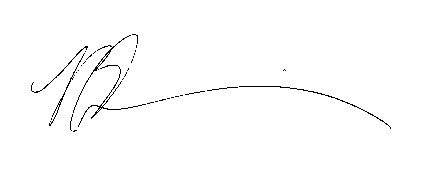
\includegraphics[height=1.5cm]{images/Barry.jpg}


\newpage

\chapter*{ACKNOWLEDGEMENTS}
\addcontentsline{toc}{chapter}{Acknowledgements}
% Don't change anything above this.
% We do not number this or add it to the contents!
% Overly long acknowledgements are not professional

The sun rises from the East and sets in the West. This would not be the case if the earth does not orbit around it. Just as the sun, this work has been made possible by different parties. First of all, I would like to thank the Almighty for giving me the strength and courage to finish the project. African Institute for Mathematical Sciences (AIMS), saw the potential in me, and gave me a platform where I would learn and bring out the best from my potential. I will forever remain grateful for this opportunity. I would also like to pass my special thanks to Barry C Sanders, my supervisor, who  supported me very much in this new area of study. His tireless efforts to explain new concepts and give constant feedbacks cannot go unnoticed. The first time I heard the name tutor I did not actually know what it really means. Today it means sacrifice, continued support and service to the people. This was the meaning given by my tutor Edward. I lack words to express my gratitude to him. Lastly I would like to thank my fellow colleagues and everyone who contributed to my success.
\newpage
\chapter*{DEDICATION} 
\addcontentsline{toc}{chapter}{Dedication}

I would like to dedicate this work to my family, always my number one funs.

% Abstracts are usually written in English, with a version in your
% mother tongue underneath
\chapter*{Abstract} 
\addcontentsline{toc}{chapter}{Abstract}
% Don't change anything above this.
Imagine you have limited computational capabilities and you wish to delegate tasks. You want to be in a position where only you can access, read and interpret the data. Homomorphic Encryption is a scheme that allows computation on encrypted data. The journey to achieve homomorphic encryption and the progress that has been made to date is presented here. We have both Classical Homomorphic Encryption and Quantum Homomorphic Encryption. In classical both the client and server are classical while in quantum the client is classical and the server is quantum.  Quantum Homomorphic Encryption has several advantages over Classical Homomorphic Encryption like some tasks that are considered to be hard can easily be performed. A vivid description on how both work is explained in the essay.

% At a unviersity like Stellenbosch you *must* produce an abstract in Afrikaans for your masters.
% At AIMS you are encouraged to repeat the abstract in your mother tongue
% French, Igbo, Mlagasy, etc. just write it using LaTeX's special
% characters.
% Arabic students see the arabic.tex file for an example
% Amharic use openoffice and export from there and import a figure here.
% Where the words do not exist put the English work in italics, or use mathematical symbols.





% Don't go typing out the contents.
\tableofcontents
\newpage
% We switch to arabic numerals here where your page count starts
% Essays must be 35 pages long *starting here* and up to and including
% the conclcusion. It does not include the acknowledgements or references.
% 
% Figures may differ between topics, but they are not there
% to fill the pages -- they must add meaning.
% In general most figures should be 0.8 times the width of the page
% (perhaps wider in total when two or three columns of figures)
% See the example in chapter one for defining that. Be *consistent*
% in your presentation of information.
\pagenumbering{arabic}
\pagestyle{myheadings}
%-----------------------------------------------------------------------------
% Each chapter goes in a separate file
% Chapter titles are just examples
% Always have a question
% Note the Case Pattern used at AIMS
\chapter{Introduction}
\section{Overview}
Owning a computer was the new thing in the world. Everyone wanted to have one. The first computers were very large in size but as the years passed by, the size decreased. We now have portable computers. Computers may crash and we lose all our data, or the computation we want to perform, our computers cannot handle. A need arose to increase storage space and processing power. We would not always be purchasing new machines and training staff all the time as the needs changed everyday.  Thus we required to store and process our data elsewhere in addition to the local storage. This was characterized by Cloud Computing. Cloud Computing can be described as using the cloud (some server stored somewhere anonymous) to carry out tasks like storage and data management over a network rather than doing it in our own computers.  

We enjoyed cloud computing for a while but then the issue of security came along. A user does not have control of whom would access his/her data while in the cloud. Mischievous users may intentionally or accidentally get hold of someone else's data. One can imagine a leakage of a patient's examination results or diagnoses. It started by using for example a symbol to represent a patient. Yes the patient's name may be anonymous, but if someone has access to the hospital's data, they would know how many people are suffering from a certain disease among others. This user can decide to cause unnecessary chaos or theft in case of a bank where a customer's personal information such as credit card pin code is accessed. It became possible to encrypt data and store it but performing computations on this encrypted data was not possible. Encryption is simply using a different representation of data for instance using 123 to represent the word transform. Only someone who knows how to interpret it can use it.
 
Homomorphic Encryption shows that it is actually possible to perform computations on encrypted data.

\section{Background and Motivation} 
In April 2011, a Play Station's network owned by Sony was hacked. There was exposure of customers information like credit card and passwords. The responsibility for this incidence was accepted by Sony. They realized that they had not done enough to ensure security of their customers' data. They would have encrypted it before storage. In this same period researchers also discovered that files in Dropbox were stored unencrypted. This lead to users leaving and closing their accounts with Dropbox since they felt insecure.  

According to, ensuring security would be done at different levels. Securing the hardware (this is the physical system), software (set of instructions executed in the system) and the data itself. In the hardware, locks were put to limit access to unauthorized persons. Systems to detect an intrusion and devices that verify persons identity were put into place. In the software, programs that limit access to database and protect one user from other users were developed. Also, software programs were written in such a way that their weaknesses could not be easily exploited. Password checkers and virus scanners application programs were also developed. The solution to the data was encryption. Data is only useful to parties if it can be readable and interpreted. Encrypted data is only useful if one can decrypt it.  All this assured the user of security. At the instances where the user needed to use the data then there was a problem because the data needed to be decrypted before any form of computations. This raised a security issue again. We needed to develop a system that allows computations on encrypted data. This is known as Homomorphic Encryption. This assured the user of total security. 

Previous works have been done trying to explain how Homomorphic Encryption can be implemented on various platforms using different types of data. In 2013  tried to explain a model which encrypts hospital data. After the computations are done the number of patients suffering from a certain disease is returned in an encrypted format. The hospital's management then decrypts it. Showed a system where different people are using it to perform an optimization problem among themselves. An optimization problem is a problem where you want the output to be the maximum based on certain inputs, for example maximum profit. The task is to find the inputs. These people work without revealing any information about their inputs to the server. Using a similar approach to these works, we will discuss possible applications of Quantum Homomorphic Encryption using example use cases.


\section{Aim and Objectives of the Study}
Imagine you own a business and you want to charge different prices to different people based on their financial capabilities and customer loyalty. Your resources are limited thus you have to outsource resources such as storage. You do not want this information to leak to the public since this may make some customers to withdraw. You want to maintain the privacy of this information. The system should be able to determine the financial status and loyalty of a customer then charge accordingly. No information about the customer is revealed or the prices charged to other customers.

The aim of this essay is to show the current state of security while requiring services from an untrusted server. The objectives include explaining vividly the security concerns and showing steps taken to counter these issues. This is done by discussing about classical computing with its limitations compared to quantum computing. We will also see the different ideas quantum computing brings about which makes it attractive compared to classical computing, the process of Quantum Homomorphic Encryption in details and application examples.

\section{Purpose of the Study}
There was a time when bank robbery was the order of the day. Banks solved this issue by putting so many security measures such as several locks and authentication before accessing where the actual money was. Banks also required several people to approve before large transactions were made. In 2017, three men dug a tunnel for six months into a Kenyan bank and made away with 50 million Kenyan shillings which is approximately 500,000 US dollars. This shows that security issues cannot be solved 100 percent. A determined person will always find a loophole. How can we ensure that the loopholes are not easily discovered and exploited?

The purpose of this essay is to show how computing security has evolved over the years, the steps and measures taken in different settings using the resources available, the plans under way to secure the data and computing in future and the new discoveries especially Quantum Computing and its effect on computing security. We will also see why one would consider a Quantum Homomorphic Encryption over a Classical Homomorphic Encryption. 

\section{Organization of Essay}

This essay is subdivided into five different chapters. In Chapter 2 we will discuss about classical and cloud computing with their limitations compared to quantum computing. In Chapter 3, quantum computing is vividly discussed. Different types of encryption in quantum computing and why one is chosen over the other are also discussed. Chapter 4 talks about examples of use cases where Quantum Homomorphic Encryption could be used. Chapter 5 contains the conclusion with recommendations.

%Explain the context of your essay topic, so that the
%topic itself appears motivated, natural and important.
%
%\begin{figure}[h]
%\psfrag{A}{$d^2$}
%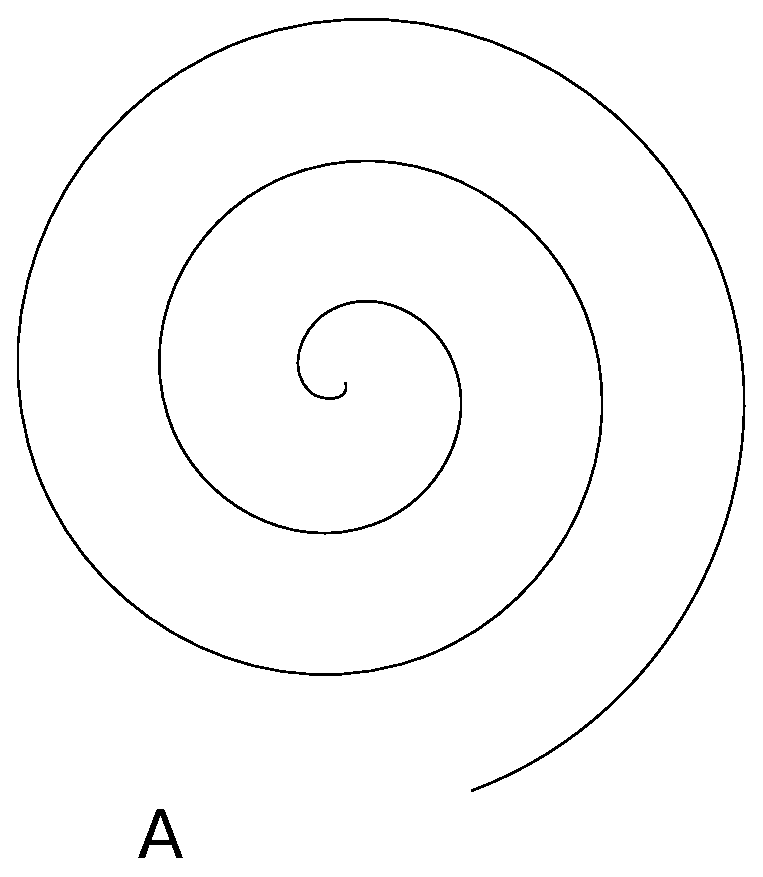
\includegraphics[scale=0.5]{images/drawing.eps}
%\end{figure}
%
%Paragraphs are separated by blank lines in the \LaTeX\ code, 
%and the line spacing, paragraph indentation,
%and paragraph spacing are set in the preamble for you, 
%according to AIMS house style.
%
%This is a textual citation \citet{shannon44}. And this is a parenthetical citation \citep{shannon44}. You probably want to use the latter more often.
%
%\section{Moving On}
%Let's demonstrate a figure by looking at Fig.~\ref{bandwidth}. 
%
%\begin{figure}[!h]
%% Use "\centering" in floats (figure, table), but if you need to center
%% some text (why?) use "\begin{center}...\end{center}".
%\centering 
%% Figure environments same as 0.8 * \textwidth please
%% That does not necessarily mean the actual picture size,
%% it is a guideline for the environment which could contain
%% 2 or more pictures! Be consistent and follow the guidelines
%% provided in your sources.
%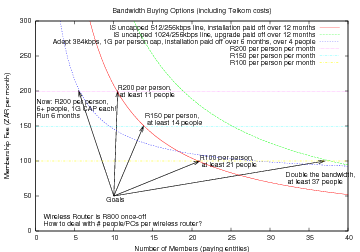
\includegraphics[width=0.8\textwidth]{images/bandwidth-colour.png}
%\caption{Planning community bandwidth sharing costs. 
%  Note caption capitalization.}
%\label{bandwidth} 
%% if you move the label it breaks the reference numbering; 
%% always have it *after* the caption.
%\end{figure}
%
%Remember how to include code with {\tt verbatim} 
%and to fix the tabs in {\sf python} in a verbatim environment? 
%It may be best to have an `include' command for code, 
%not to have to re-edit it all the time.
%\verbatimtabinput{code/mycode.py}
%
%
 % Introduction is usually a chapter itself.
\chapter{Classical and Cloud Computing}
In this chapter we will discuss about classical computing and its limitations compared to quantum computing.
\section{Classical Computing}

The probability of making errors is very high by hand. A computer is a universal machine. A universal machine can be described as an electronic device with the ability to solve problems. These problems have solutions, that can be represented by a set of instructions. These problems are known as computational problems because the classical computer can solve them. 

Computational problems include decision problems, search problems, function problems and optimization problems.  Decision problems are similar to making a choice between true or false, where true can be represented by 1 and false 0. Search problems are like looking for a word in a text. Function problems are for example evaluating $\cos (\theta)$. Optimization problems are problems whereby, you want the output to be the maximum possible value. We therefore find the inputs which satisfy this condition. What prices will you charge the customers in order to make maximum profit without exploiting your customers?

Computers can be connected to each other in order to communicate. This is known as distributed computing. Each processor has its own memory but can communicate with others by sharing messages. One memory can also be shared by multiple processors (parallel computing). Parallelism speeds up computations since different tasks can be performed at the same time. The more the number of processors the more expensive a machine is. 

To solve problems, a computer requires resources. The more resources required the more complex it is described. Thus computational complexity is defined by the resources used. A client may wish to perform tasks which require computational power beyond their capabilities. They may also have limited resources, therefore, they decide to outsource resources from remote servers. The client therefore delegates tasks. Can the client trust the output from the server? If the client cannot trust the server, then this raises a reliability issue. One of the solution to this issue is that, the client can choose multiple servers provided atleast one of them is reliable (honest) and delegate tasks to them \citep{canetti2011practical}. The problem with this protocol is that, it is difficult to determine which server is honest. This makes verifying correctness to be based on probability. This can be done by a client dividing the task into stages. The client can therefore access the output of each stage. This allows the client to check for inconsistencies between the servers' outputs. In case of inconsistencies and if the stage affected can easily be performed by the client, then determining the dishonest server becomes simple otherwise it would be very difficult. There are times when a client requires urgent results. During these times, the client may have no time to compare outputs from different servers. Requiring services from different servers is expensive and time consuming.

Servers could decide to give false results (dishonest) based on a couple of reasons. The resources required to perform the computation may be a lot to the server. This makes the profit made less than the estimated one. The server could also benefit from some outputs for example poll results. An employee could just decide to interfere with the computations being executed \citep{canetti2011practical}. 


Cloud computing is an example of a delegated computing system.


\section{Cloud Computing}
\subsection{What is Cloud Computing?}
Cloud Computing is the process whereby, computation is done somewhere else (in the cloud), and is similar to working on your personal computers \citep{hayes2008cloud}. Cloud is some server stored somewhere anonymous only the service providers knows about its whereabouts. Clients for example companies or individuals are able to request services such as storage, manipulation of data and computations among others. Cloud services are offered as demanded by the clients. Clients do not have to train their staff, worry about data loss in case of system crashes, buy new infrastructure or get licenses for softwares.

The three major types of cloud computing services are: Platform as a Service (PaaS) such as Google App Engine (which is mainly used by developers), Software as a Service (SaaS) for example email and Facebook and Infrastructure as a Service (IaaS) like storage facilities and servers.

Examples of companies offering cloud services include Amazon, Google and IBM.

The main disadvantage of cloud computing is security on \citep{subashini2011survey} and \citep{miller2008cloud}. 
Security is one of the issues that is making some companies to shy away from cloud computing. Most governments have rules that their sensitive information should not leave their respective countries. The cloud servers may be located anywhere in the world. In cloud computing data may be changed and this interferes with its integrity. Integrity can be defined as the quality of wholeness. Data which has been changed is not whole. Data could be changed to manipulate intended results. Duplication of data could also occur. This amounts to information theft. In cloud computing making an exact copy of data is possible and the client may not learn about it in good time. Data can be interfered with. Since many clients are using the same server, the possibility of their data mixing up is very high. Some clients could also be malicious and interfere with other client's data. Leakage may also occur. Sensitive information may be exposed to unintended audience. For example, if a user receives emails from different people but always performs a search on a specific sender, this could reveal to the server that this person has a level of importance to the client. The server may exploit this loophole to gather information on why this person interest the client.

The bottom line is, we do not trust the server. Our privacy, confidentiality and integrity is put at risk. The data may end up falling into the wrong hands with unauthorized personnel which would lead to severe consequences. Organizations whose data is mainly sensitive information, would find it hard to adopt cloud computing. A user can encrypt data before storing it in the cloud and when he/she needs it they can download and decrypt it. Thus, this user cannot use other services apart from the storage. Other costs of hardware and software, which will be used to process the data are incurred \citep{yang2013evaluation}.

A solution to this is homomorphic encryption, whereby a server performs computations on encrypted data.

\section{Classical Homomorphic Encryption and its Limitations}
Homomorphic Encryption is also an example of a delegated computing system. This system ensures secure delivery of information, storage and computations. Homomorphic encryption is the ability of a server to work on encrypted data. According to \citet{ogburn2013homomorphic}, homomorphic encryption can either be partial, somewhat or fully. In Partial Homomorphic Encryption, you can either perform addition or multiplication on encrypted data but not both. A Somewhat Homomorphic Encryption technique has the ability to perform both multiplication and addition on limited numbers. A Fully Homomorphic Encryption can support both multiplication and addition and is not limited to any numbers. Most of us would choose a Fully Homomorphic Encryption system. Its only disadvantage is that, it is less efficient as compared to Partial Homomorphic Encryption and Somewhat Homomorphic Encryption. 

Figure \ref{fig1 : Encrypt} is an example of a Homomorphic Encryption. The words are concatenated after encryption. The result obtained after decryption, is the same with the result if the concatenation was performed without the encryption.
\begin{figure}[!h]
\center
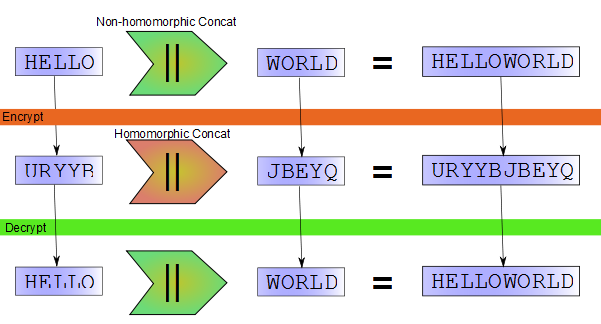
\includegraphics[scale= 0.5]{images/encrypt.png} 
\caption{Encrypted concatenation}
\label{fig1 : Encrypt}
\citep{Craig}
\end{figure}

\subsection{Why is Homomorphic Encryption considered secure?}
As it can be seen from Fig \ref{fig1 : Encrypt}, no information is revealed to the server. The server can learn about the information only if it can decrypt it. The server can only decrypt the information if they know how you as the client encrypted it and they possess the decryption key. This may be termed as negligence from the client's side. In Homomorphic Encryption the integrity of the data is maintained. How will the server change something like 'JBEYQ' which they can't even interpret? The client may get some results and tell that something is wrong, in case the server changes something. It is very easy to manipulate something that you can understand but difficult otherwise. Data cannot be duplicated. The encrypted data can be duplicated but the real unencrypted data cannot. Sensitive information cannot leak too. Privacy and secrecy are also maintained.

\subsection{Limitations of Classical Homomorphic Encryption as compared to Quantum Homomorphic Encryption}
We always seek to improve the existing things. The big question is why Quantum and not Classical?	A classical computer is limited in terms of computation power as compared to a quantum computer. Some tasks like factorization that can be performed easily on a quantum computer are hard and require a lot of time on a classical computer \citep{unruh1995maintaining}. The main idea is to improve speed and efficiency. This is especially when dealing with large chunks of data like performing a search operation in a large database and factorization of large numbers. 

This makes Quantum Homomorphic Encryption attractive. 

%First of no information about the data is revealed unless the server can decrypt it.
 % Chapters might go from 2. problem statement, 
                 % through 3. model, to 4. analysis & results
\chapter{Quantum Computing and Quantum Homomorphic Encryption}
In this chapter we discuss what quantum computing and Quantum Homomorphic Encryption entails. 

\section{Quantum Computing}
In Quantum Computing, we have quantum bits (qubits) represented as $|0\rangle$ and $|1\rangle$  as opposed to the classical bits (0 or 1) in classical computing.  We also have quantum logic gates namely Hadamard (H), Z, X and CNOT which form the backbone of quantum computing. The gates can be represented as follows using circuit diagrams:
\begin{figure}[!h]
\center
\begin{minipage}[b]{0.3\textwidth}
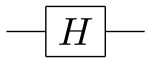
\includegraphics[scale=0.75]{images/hadamardgate.png} 
\caption{Hadamard gate}
\label{fig: Hadamard}
 \end{minipage}   
\hfill
\begin{minipage}[b]{0.5\textwidth}
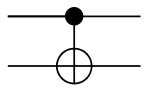
\includegraphics[scale=0.75]{images/cnotgate.png}  
\caption{CNOT gate}
\label{fig: CNOT}
\end{minipage}
\center
\begin{minipage}[b]{0.3\textwidth}
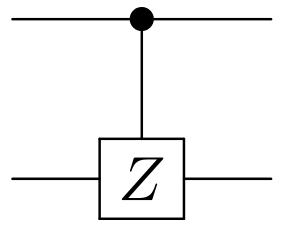
\includegraphics[scale=0.45]{images/zgate.png} 
\caption{Z gate}
\label{fig: Z}
 \end{minipage}   
\hfill
\begin{minipage}[b]{0.5\textwidth}
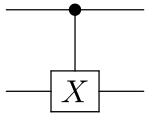
\includegraphics[scale=0.75]{images/Xgate.png} 
\caption{X gate}
\label{fig: X}
\end{minipage}
\end{figure}

The two main ideas brought about by quantum computing are superposition and entanglement which are adopted from quantum mechanics. If any computation uses these two mechanisms it is known as quantum computing. In quantum computing, a zero and a one can be represented simultaneously. This is known as superposition. It saves on processing time. For example, you have a box full of white chalks, but, you have one green chalk that you want to obtain from the box. The box is not transparent hence you cannot see what is inside. To solve the problem classically, you have to pull one chalk at a time until you get the green one. Quantum permits you to hold all the chalks at the same time and use probability to pull out the green chalk. This is the idea brought about by superposition.

Entanglement is when two particles interact and acquire states of each other, thus the output will be a mixture of the interacting particles, hence to describe one particle one has to refer to the other. To illustrate an entanglement, let us use a Hadamard and a CNOT gate. A CNOT gate is a Controlled NOT gate. If the control is a qubit of one then we apply a NOT to the bit in the target, otherwise nothing happens. This is shown in Figure \ref{fig:entanglement} below.

\begin{figure}[h]
\center
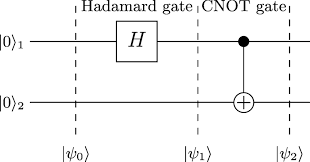
\includegraphics[scale=1]{images/entangle.png} 
\caption{An entangled circuit}
\label{fig:entanglement}
\end{figure}

At $|\psi_0 \rangle$ we have the output as $|0\rangle _1 |0\rangle _2$. It can also be written as $|0_1 0_2 \rangle$. We have $|0\rangle _1$ qubit passing through the Hadamard gate (H). By definition
$H|0\rangle =| \overline{0} \rangle = \dfrac{|0\rangle + |1\rangle}{\sqrt{2}}$. $|0\rangle _2$ does not change. The output $|\psi _1 \rangle $ is $ \bigg(\dfrac{|0\rangle + |1\rangle}{\sqrt{2}} \bigg)|0\rangle = \dfrac{|0\rangle_1 |0\rangle_2 + |1\rangle_1 |0\rangle _2}{\sqrt{2}}$. We then pass through the CNOT. Since $|0\rangle_1$ is 0, $|0\rangle_2$ remains unchanged, $|1\rangle_1$ is 1 hence $|0\rangle _2$ flips to $|1\rangle _2$. Thus the output $|\psi_2 \rangle $ is $\dfrac{|0\rangle_1 |0\rangle_2 + |1\rangle_1 |1\rangle _2}{\sqrt{2}} = \dfrac{|0_1 0_2\rangle + |1_1 1_2\rangle }{\sqrt{2}} = \dfrac{|0 0 \rangle + |1 1\rangle }{\sqrt{2}}$.

This is a maximally entangled state.

Quantum computing also supports parallelism. As opposed to classical computing where different processors are required, quantum computing parallelism is done on the same chip. As long as the tasks are related, they are carried out at the same time.

\section{Approach Techniques}
The properties of quantum computing enable computations to be performed on encrypted data (hidden).
This is the ability for a server to process data delegated to it, without accessing it. 
The two types of techniques used are Blind Quantum Computing and Quantum Homomorphic Encryption.
Blind actually means you cannot see. This encryption uses the same application. The server is blinded from input, output and computation. This is a technique where the server performs computations they do not know of on encrypted data and produces results which they do not also know from an encrypted input. Sounds hilarious right?
Quantum Homomorphic Encryption is a technique where the server performs computations they actually know of on encrypted data, that is, the input and output is encrypted but the computation is known.

\subsection{Differences between Blind Quantum Computing and Quantum Homomorphic Encryption}

\citep{broadbent2009universal}, \citep{fitzsimons2017private},\cite{ouyang2015quantum},\citep{Joe}

\begin{table}[!h]

\begin{tabular}{|c| c| c|}
\hline
 & Blind Quantum Computing & Quantum Homomorphic Encryption\\
\hline
1 & Everything is encrypted &   Only the input and output\\ 
 & (input, output and computation) &  are encrypted.\\
 &\citep{huang2017experimental} (abstract). &  \citep{broadbent2015quantum} (Introduction).\\
\hline
2 & Uses information theoretical security & Uses computational security protocol\\
  & protocol (can not be broken in) & (it is hard to break in).\\
  & \citep{fitzsimons2017private} (pg1).&  \\
\hline
3 & It is possible to expand the system & The system is fixed \\
& based on the client's needs &  \\
& \citep{Joe}.& \citep{Joe}.\\
\hline
4 & An interference with the protocol is usually & No measures are put into place hence there is a \\
  & detected because measures are put into place &  probability that an interference can go undetected.\\
  & \citep{broadbent2009universal}(abstract). & \\
\hline  
\end{tabular}
\caption{Differences between Blind Quantum Computing and Quantum Homomorphic Encryption }
\label{fig:table1}
\end{table}

\subsection{Why Choose Quantum Homomorphic Encryption Over Blind Quantum Computing?}

Information theoretical security used in Blind Quantum Computing is very hard to implement on a classical client hence its implementation is very expensive \citep{ouyang2015quantum}.  You cannot break into a system using information theoretical security even if your computational power is greater than the system. Due to the high cost  of implementation, very few clients will afford it. In most Blind Quantum Computing protocols, the client has some quantum computation requirements, though protocols that do not have this requirement exist \citep{broadbent2009universal}. This makes us choose Quantum Homomorphic Encryption which uses computational security which is hard to break in. Thus the risk of an adversary attacking the system is low.

\section{Quantum Homomorphic Encryption}
As seen earlier, it is possible to delegate tasks (data processing) to a server while the access to the data is not given away. The ability of a server to perform computations on encrypted data solves our security issue.  

\subsection{How the security issue is solved in Quantum Homomorphic Encryption?}


Since the server does not know the input or output it is impossible to change data to manipulate results, also, the integrity of the information is upheld. Data cannot be duplicated because, in quantum, duplication involves measurement and this changes the state thus you will never get the exact copy \citep{kassal2011simulating}. Quantum Homomorphic Encryption as we saw earlier, uses computational security. It is very hard to break or attack the encrypted data. To break in you require a lot of time. This makes it almost impossible for sensitive information to be leaked.


\subsection{How does Quantum Homomorphic Encryption work?}

There are four stages involved namely: Key generation, Encryption, Evaluation and Decryption \citep{broadbent2015quantum}.

All these stages are performed by the classical client . 

\subsection{Key generation and Encryption} 
Key generation produces a pair of public and private key. The public key is used to encrypt data while the private decrypts it. Key generation can be done using the RSA method. While using a computer program such as Python, an already existing RSA module exists. This implies that the client inputs a number and a pair of public and private key is generated. 

RSA can also be done using a mathematical approach. Two random large prime numbers say $p$ and $q$ are chosen. Let us take $p = 17$ and $q = 11$. We then calculate $N = p\times q$, $17\times 11 = 187$. $N$ is the system modulus.  The factorial of $p$ and $q$ is then calculated to find the public key which is used for encryption. In our example, we get the factorial as follows $(17-1)(11-1) = 16 \times 10 = 160 = 2^5 \times 5$. We now choose a number $e$ that does not divide any factor of $(p-1)(q-1)$. We can take our $e = 3$ as $3$ does not divide either $10$ or $16$. Thus $3$ is our public key. To get the private key we multiply our public key with a number say $d$ such that $ 1 = e \times d \mod (p-1)(q-1)$. We therefore calculate $d$ as follows, 
\begin{eqnarray*}
e \times d &\equiv & 1 \mod (p-1)(q-1)\\
3d &\equiv & 1 \mod 160\\
3d &=& 1 + k\cdot 160 \\
\end{eqnarray*}
$k$ is any random number that satisfies the equation. If we let $k =2$, then $d = 107$. Thus our private key is $107$ \citep{meissen2012mathematical}. Encrypted data can be referred to as a cipher text while unencrypted data is called a plain text. A plain text is transformed into a cipher text using the public key. Cipher text = (plain text)$^e \mod N$ while the plain text = (cipher text)$^d \mod N$.

The client can generate as many key pairs as they want to. This means that different public keys can encrypt the data producing different forms of encrypted data. The client is in a position to choose randomly which encryption to send. Since in homomorphic encryption the computation is known to the server, if you always send a certain encryption to perform the same computation, it would be easy for the server to start guessing. Also, if the server knows that different encryptions represent the same data, then it would be easy to guess too.

For example, you delegate the server to perform factorization. Factorization problems are easy to verify when given the results but hard to solve. It is very difficult for the server to know exactly which number you are factorizing since the input and output are encrypted. The computation does not reveal sufficient information about the input and output which would make an attack easy, apart from the input is a number and the outputs are prime numbers.

How many numbers and prime numbers exist? Will the server start guessing one by one? How long will it take for the server to actually guess the  correct number? It is possible for the server to guess the correct number but the probability is very low maybe 1 out of a million trials \citep{yang2013evaluation}.

\subsection{Evaluation and Decryption}
After key generation and encryption, we then evaluate. This is checking the correctness of the algorithm. The public key encrypts the already existing cipher text to produce another cipher text. For example let us encrypt \textit{g} in mod of a prime number say \textit{p}. Then we encrypt it again in$\mod 2$. Our cipher text reads c = (\textit{g} mod \textit{p}) mod 2. We first decrypt c in$\mod 2$ using the public key to check whether we will get \textit{g} mod \textit{p}. If we get the desired result then the algorithm is correct.  However the time taken to evaluate and the overall cost should be less than the individual cost of key generation, encryption and decryption. 

We have our cipher text and private key, we combine them to produce the plain text. Plain text = (cipher text)$^d \mod N$. This is our decryption process. The decryption  is done by the client after they receive the results of the delegated task \citep{ouyang2015quantum}.



 % You do not need to have exactly 4 chapters.
                 % It is probably a good minimum, with 5 chapters 
                 % average, and 7 chapters might be a maximum.
\chapter{Applications}
In this chapter we will discuss examples of places where Homomorphic Encryption would be used. This section seeks to review already existing proposals and use cases.

\section{School Example}
\begin{figure}[!h]
\center
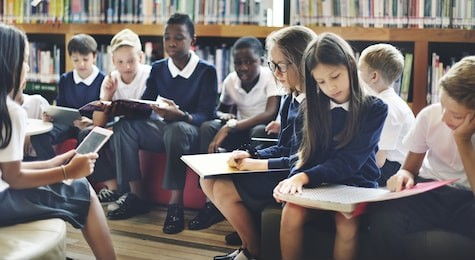
\includegraphics[scale=1]{images/school.jpg} 
\caption{Students in the library.}
\label{fig1: School Example}
\citep{archerapplications}

\end{figure}

We are familiar with students dropping out of schools based on different reasons. For example not everyone who joins graduate school makes it for graduation. The reasons for dropping out vary from one student to another. In some areas, most girls drop out in high school due to early pregnancies. What factors lead to early pregnancies? Peer influence, lack of proper guidance or adventure could be some of the reasons. Other reasons that could lead to school dropout may include illnesses, lack of school fees and psychological issues. 

We aim at reducing the number of school dropouts. We want to make predictions of a possible dropout before it actually happens. This will enable us to find a way to best assist the student as the Ministry of Education. Predictions are made based on statistics which means that we have to access the students data. We are dealing with all the schools for example high schools. This implies that the data should be stored in a central place. 

We do not fully trust the server. We also do not trust the other parties who may be using the server. No school is given access to another school's data. In some instances, the school may not have sufficient information to make a prediction. These are cases where for example, a sickness may be the cause of a dropout. This means that we require information from a hospital. We may also require information from different hospitals if the student has sought medication from more than one hospital. 

Another scenario is when a student drops out due to lack of school fees. We may need to check the financial status of the parents or guardian. This implies that banks and welfare services would be of great help. Different institutions therefore need to be integrated into the system. This makes it even more difficult. The schools may be reluctant to provide private information about the students due to laws that govern them. The central place where information is stored could be a potential target for attackers \citep{archerapplications}.

Homomorphic Encryption provides a solution to most of these problems. Data is encrypted before storage and computations are performed on the encrypted data. This ensures data sharing without breaking the laws. It also reduces the risk of an attack on the database. Data is encrypted in storage and also in transit. Different schools and sectors encrypt their data differently. They all use for instance, the RSA method, but have different public and private keys, therefore, no institution can decrypt another institution's data. As a result no single institution can access the whole data. We may also use secret sharing as an additional security measure to allow any computation. Secret Sharing as the name suggests, is the process whereby, authorization requires different pieces to be put together. The pieces are held by different people such that all combined can access the database, but an incomplete number of persons cannot. A good example is in a bank where a large transaction must be authorized by different people before it is processed. This builds the confidence  and a sense of ownership to the parties involved. We also ensure that the minimum number of persons  who can authorize involve persons who cannot collude. 

The first step is that different parties should approve access of a party to the database. After access is approved, a query is made to the server. The query is encrypted but the server knows the computation it is going to perform for example search function. Data about a specific student is accessed from different access points like a hospital and school. The data from these two places is encrypted differently and may be stored in different databases. If for example we get data from the school which shows that a student has been constantly sent home as a result of failure to pay school fees, we can query about the bank details. After the data is retrieved, it is then merged. A prediction is therefore made from the merged data based on the characteristics or the model used. Batch requests can also be made such that the dropout risk of students from an institution is performed simultaneously. 

This could be slow using a classical server and can even take days for a query to be processed. We therefore recommend a quantum computer as a server as it is fast and efficient. 


\section{Hospital Example}
Information about a person's health is usually sensitive and medical practitioners swear an oath of secrecy. This information should be protected at all costs to avoid leakage which may cause damage both to an individual and the institution itself. Researchers or the medical practitioners would want to use this data to conduct a research about a certain drug and its effect to the patients. They may also want to use the data for better planning or to predict an outcome. All these should be done while preserving the privacy of the patient.

\citet{archerapplications} describes a use case where the doctors record patients' details like blood group, genotype, signs and symptoms, lab test results, drug prescription and the efficiency of the medication administered. This is done over a period of time. The data is then encrypted and stored in the database where the server is not fully trusted as shown in figure \ref{fig1: Hosptial Example}. 
\begin{figure}[!h]
\center
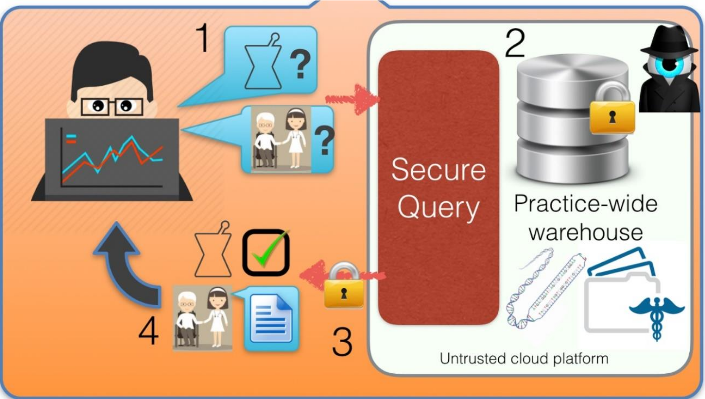
\includegraphics[scale=0.5]{images/hos.png} 
\caption{Hospital Example }
\label{fig1: Hosptial Example}
\citep{archerapplications}
\end{figure}

For cancer patients, the tumors differ from one patient to another. This implies that the treatments  also differ and patients may also react differently to the medication. The reaction may depend on things like the size of the tumor, allergic reactions and genes just to name a few. The details of different patients are already in the database. If a new patient visits the hospital the doctor queries the database based on the patient's details that are similar to those stored in the database, which may include signs and symptoms among others.
The query is encrypted but the computation is known to the server. After getting the results, the doctor decrypts and knows the best treatment to administer to the current patient based on different past results. This saves on time required to test the medication that would work on the patient. The patient requires to pay the bill after treatment. To pay the bill things like tests performed, diagnosis and prescription are exposed to the cashier. This could lead to leakage. Using homomorphic encryption, the amount could just be calculated and the payment made without exposing any additional details.

According to \citep{naehrig2011can}, the data stored about the patients can also be useful in several ways. Based on the patients data, functions would be computed to determine certain risks such as possibility of a re-infection and attacks like hypertension. Alerts are then sent to the doctor and the patient. The patient is hence in a position to act accordingly before the risk becomes a reality and safety precautions taken. This improves the efficiency of the services provided by the hospital. 

This argument is based on a classical client and a classical server. It can be implemented using a classical client and a quantum server as we have earlier seen the advantages of quantum computing over classical computing for instance speed and efficiency. This use case would therefore work best using Quantum Homomorphic Encryption.


The school and hospital use cases can also be implemented using Blind Quantum Computing. As we saw earlier, its main disadvantage is cost of implementation. This makes Quantum Homomorphic Encryption our most preferred option.



    % Conclusion is usually a chapter itself. 
\chapter{Conclusion and Recommendations}
Security and privacy are the two most valued priorities among the many things we regard as
 important. When selecting a house location, we often put security as the major factor of consideration. You do not want someone to intrude your privacy or walk away with your hard earned cash or favorite items. Before telling our friends and family members something about ourselves we always consider whether they are in a position to keep it to themselves or not. We apply for jobs where we expose a lot of our details. We remain hopeful that none of this information will fall into the wrong hands. For instance, most ladies want to hide their age. After providing their information, they trust that the institution will handle it in a very secure and private manner.

There is a time people did not believe that we would actually have computers. Look at the way technology has change the world! Personal computers could no longer handle our problems. We needed to replace them with better machines which was expensive for large organizations. We therefore required to outsource resources. Cloud computing came along and we enjoyed it for a while until the issue of security popped up. There have been numerous trials to solve this issue like having several authentications before being granted access. The most interesting solution so far is Homomorphic Encryption. One can store, process and transmit encrypted data while still maintaining its confidentiality, privacy and security.

In this essay, a solution to the security issue while outsourcing and requiring services of untrusted server has been presented. Homomorphic Encryption is the process where by, computations are performed on encrypted data. The different solutions tried before Homomorphic Encryption such as multiple authentications, have their own limitations. All these solutions have loopholes like bypassing passwords which put security of the information at a risk. Homomorphic Encryption has proved to be a solution with close to no loopholes, unless someone steals your private key. A private key as we can recall is the key used for decryption. Data is encrypted in storage, transit and during computations.

Two examples, a school and a hospital are given. These are places where Quantum Homomorphic Encryption (QHE) could be useful. QHE has several advantages over Classical Homomorphic Encryption (CHE) like better computational power, speed and efficiency. Quantum states cannot also be duplicated due to their non-cloning property. Cloning involves measurement and measurement changes the state as illustrated in the essay. These advantages of QHE over CHE make QHE more attractive. A comparison between Blind Quantum Computing (BQC) and QHE is clearly outlined. The main disadvantage of BQC over QHE is cost of implementation. We want more clients to be involved thus QHE is the most attractive solution to our problem.

Clearly QHE is possible. We have seen it can be implemented using a classical client and a quantum server. The problem is, there are very few quantum computers in the world hence testing and implementation is difficult. The number of people with quantum knowledge are also few in the world. This is a major setback in this area of study. This work is mainly theoretical. We need more people to enroll in quantum courses and help develop more quantum computers. With an increase in the number of quantum computers, research and experiments will be easy to perform. Different people come up with different ideas, thus, an increase to the number of people with quantum knowledge will lead to great improvements and new innovations. This will make cloud computing environments more reliable and popular among institutions dealing with very delicate data. Major improvements can also be made in the examples given and spread in other areas not mentioned. 









 % You may have more chapters. (Use e.g. git add FILE)
%\chapter{Appendix}
\section {Python Code}
%Remember how to include code with {\tt verbatim} 
%and to fix the tabs in {\sf python} in a verbatim environment? 
%It may be best to have an `include' command for code, 
%not to have to re-edit it all the time.

\verbatimtabinput{code/facerecog.py}



% This is where we stop counting pages.
% Acknowledgements and References are not counted.
%-----------------------------------------------------------------------------
% Note the errata page is not for now, it is for use during the examination.
% Not that you're going to have any errata.
%-----------------------------------------------------------------------------
% THE BIBLIOGRAPHY 
% Bibliography styles define how the bibliography is 
% listed and formatted. This is part of the AIMS house
% style and is only changed under exceptional circumstances
\renewcommand{\bibname}{References}
\nocite{*}
\bibliographystyle{apa}
%\bibliographystyle{plainnat}
\bibliography{references}
%\addcontentsline{toc}{chapter}{References}
%-----------------------------------------------------------------------------
\end{document}
